\section{Ergebnisse}
\color{red}
\begin{itemize}
	\item besten Trainingsdurchlauf genau beschreiben $\rightarrow$ Lernrate, Loss, ...
	\item Evaluierungswerte aus diesem Durchlauf nennen und beschreiben bzw. erklären
	\item viele Bildchen :-) 
	\item Bilder aus Tensorboard
	\item Matlab-Plots und Tabellen 
    \item Threshold, Table, Plots von bestem durchgang
\end{itemize}
\color{black}

Um einen guten Klassfizierer zu bekommen waren einige Trainingsdurchläufe notwendig. Zum testen der Klassifizierer wurden diese auf einen Validierungs-Datensatz angewandt. Die anfänglichen Klassifizierer haben meist nur minimal bessere Ergebnisse als der Zufall geliefert. Durch verschiedene Anpassungen die in Kapitel~\ref{training} näher erläutert wurden konnten schließlich besser Ergebnisse erreicht werden. Einige ausgewählte Ergebnisse werden in Abbildung~\ref{fig:roc} als ROC-Kurve dargestellt. Wie man gut erkennen kann verlaufen zwei der Kurven nahe der Diagonalen. Diese zwei Klassifikatoren (2018-03-12\_22-04-38 und 2018-03-12\_22-17-46) liefern keine guten Ergebnisse. Interessant und scheinbar gute Klassifikatoren verlaufen in der ROC-Kurve links oben und sind in diesem Fall 2018-03-10\_19-16-32, 2018-03-09\_21-34-4 und 2018-04-13\_20-38-20. Die anderen Klassifikatoren können als in Ordnung eingestuft werden.

\begin{figure}[htb!]
	\begin{center}
		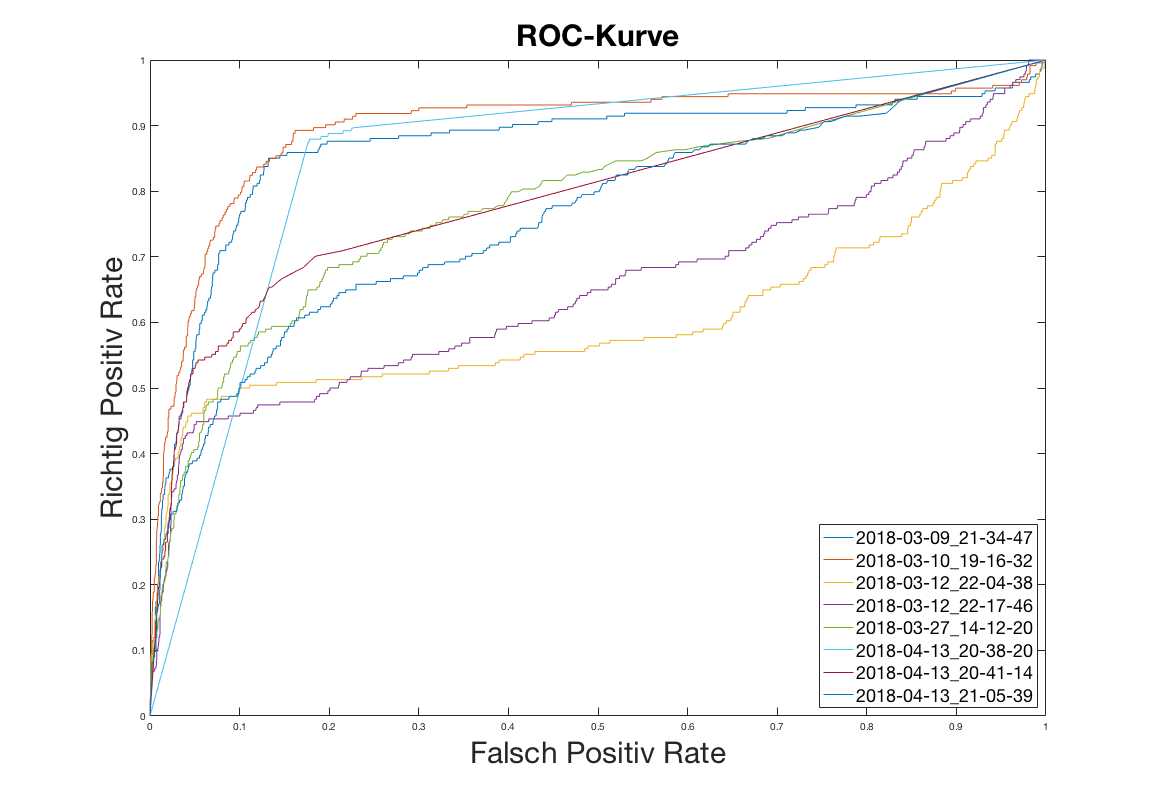
\includegraphics[width=\textwidth]{./pics/evaluation/roc_analysis.png}
		\caption{ROC-Kurven einiger trainierter Klassifizierer, angewandt auf den Validierungs-Datensatz.}
		\label{fig:roc}
    \end{center}
\end{figure}

Um die ROC-Kurve nicht optisch zu evaluieren sondern mit einem Score zeigt Tabelle~\ref{tab:auc} die Klassifikatoren aus Abbildung~\ref{fig:roc} zusammen mit ihrer AUC. Wie man gut sehen kann gleichen sich die optischen Erkenntnisse mit den AUC-Werten. Somit ist der Klassifikator 2018-03-12\_22-04-38 mit einem AUC von 0.6 der Schlechteste und nur leicht besser als der Zufall und Klassifikator 2018-03-10\_19-16-32 mit einem AUC von 0.9 der Beste. 

\begin{table}[htb!]
\begin{center}
\begin{tabular}{ll}
	\toprule
 	Klassifikator  & AUC\\
	\midrule
  	2018-03-09\_21-34-47 &   $0.87$\\
    2018-03-10\_19-16-32 &   $0.90$\\
    2018-03-12\_22-04-38 &   $0.60$\\
    2018-03-12\_22-17-46 &   $0.65$\\
    2018-03-27\_14-12-20 &   $0.78$\\
    2018-04-13\_20-38-20 &   $0.86$\\
    2018-04-13\_20-41-14 &   $0.79$\\
    2018-04-13\_21-05-39 &   $0.75$\\
 \bottomrule
 \end{tabular}
 \end{center}
  \caption{ROC-AUC Ergebnisse einiger trainierten Klassifikatoren}
 \label{tab:auc}
 \end{table}
 
Da wir bei der Hautkrebs-Erkennung noch ein paar Sonderanforderungen an den Klassifikator haben, entschieden wir uns die besten Zwei noch genauer zu Evaluieren und nahmen somit zu unserem bisher besten Klassifikator 2018-03-10\_19-16-32 auch noch Klassifikator 2018-03-09\_21-34-47 mit einem AUC von $0.87$ hinzu zu nehmen. Unser Klassifizierer soll am Ende natürlich allgemein eine hohe Vorhersagegenauigkeit haben, allerdings sollten nicht zu viele wirklich positive Ergebnisse (maligne) als negativ (benigne) klassifiziert werden. 

Tabelle~\ref{tab:scores} zeigt die verschiedenen Qualitätsmaßstäbe,  die schon in Kapitel~\ref{analysemethoden} beschrieben wurden. Wie man der Tabelle gut entnehmen kann ist Klassifikator 2018-03-10\_19-16-32 nahezu allen belangen besser als 2018-03-09\_21-34-47. Einzig und allein in der Spezifität ist er minimal schlechter.

\begin{table}[htb!]
\begin{center}
\begin{tabular}{lllllllllll}
	\toprule
 	Klassifikator  & TP & FN & TN & FP & MCC & F2 & Acc & Sens & Spez\\
	\midrule
	2018-03-09\_21-34-47 & $119$ &	$115$ &	$2406$ &	$113$ &	$0.47$ &	$0.51$&	$0.92$ &	$0.51$ & $0.96$\\
    2018-03-10\_19-16-32 & $142$&	$91$ &	$2406$ &	$114$ &	$0.54$ 	&$0.60$	&$0.93$	&$0.61$&	$0.95$ \\
 \bottomrule
 \end{tabular}
 \end{center}
  \caption{Scores der zwei besten Klassifizierer: TP = True Positives, FN = False Negatives, TN = True Negatives, FP = False Positives, MCC = Matthews Correlation Coefficient, F2 = F2-Score, Acc = Genauigkeit, Sens = Sensitivität und Spez = Spezifität }
 \label{tab:scores}
 \end{table}
 
 Da unser Klassifikator aber eher maligne Hautläsionen auch wirklich als solche Erkennen sind uns präferieren wir in diesem Fall die wenigen Falsch negativen und die mehr wirklich positive Ergebnisse, wobei trotzdem nur ein negatives Ergebnis fälschlicherweise als positiv (maligne) eingeordnet wird. Aufgrund dieser Evaluierung schließen wir also das der Klassifizierer mit dem höherem AUC, MCC, F2-Score und Genauigkeit und Sensitivität unser Problem der Hautkrebserkennung besser lösen kann. Eine etwas geringere Spezifität würden wir hierbei in kauf nehmen, wobei diese in diesem geringen Maße auch eine Zufallserscheinung sein könnte.
 
Obwohl der Klassifizierer schon von einer recht guten Qualität ist werden die Ergebnisse durch die hohe Spezifität von 95\% dennoch etwas verfälscht. Mit einer Sensitivität von $0.6$ würden wir nämlich nur $60\%$ aller malignen Hautläsionen auch als wirklich maligne klassifizieren. Im Umkehrschluss heißt das vier von zehn potentielle Hautkrebs-Vorkommen würden unerkannt bleiben. Da diese Sensitivität noch zu nah an einer Zufallsklassifizierung liegt schauten wir uns die Ergebnisse des Neuronalen Netzes des  Klassifikators noch einmal genauer an. Das Ergebnis des Neuronalen Netz ist ein Score zwischen null und eins. Liegt der Score über $0.5$ wird eine Hautläsion als maligne klassifiziert, darunter als benigne. Da wir eine höhere Sensitivität erreichen wollten schoben wir also den \textit{threshold} für eine maligne Klassifizierung weiter in Richtung null. Abbildung~\ref{fig:threshold} zeigt wie sich eine Verschiebung des Thresholds auf die einzelnen Qualitätsmaßstäbe auswirkt. 

\begin{figure}[htb!]
	\begin{center}
		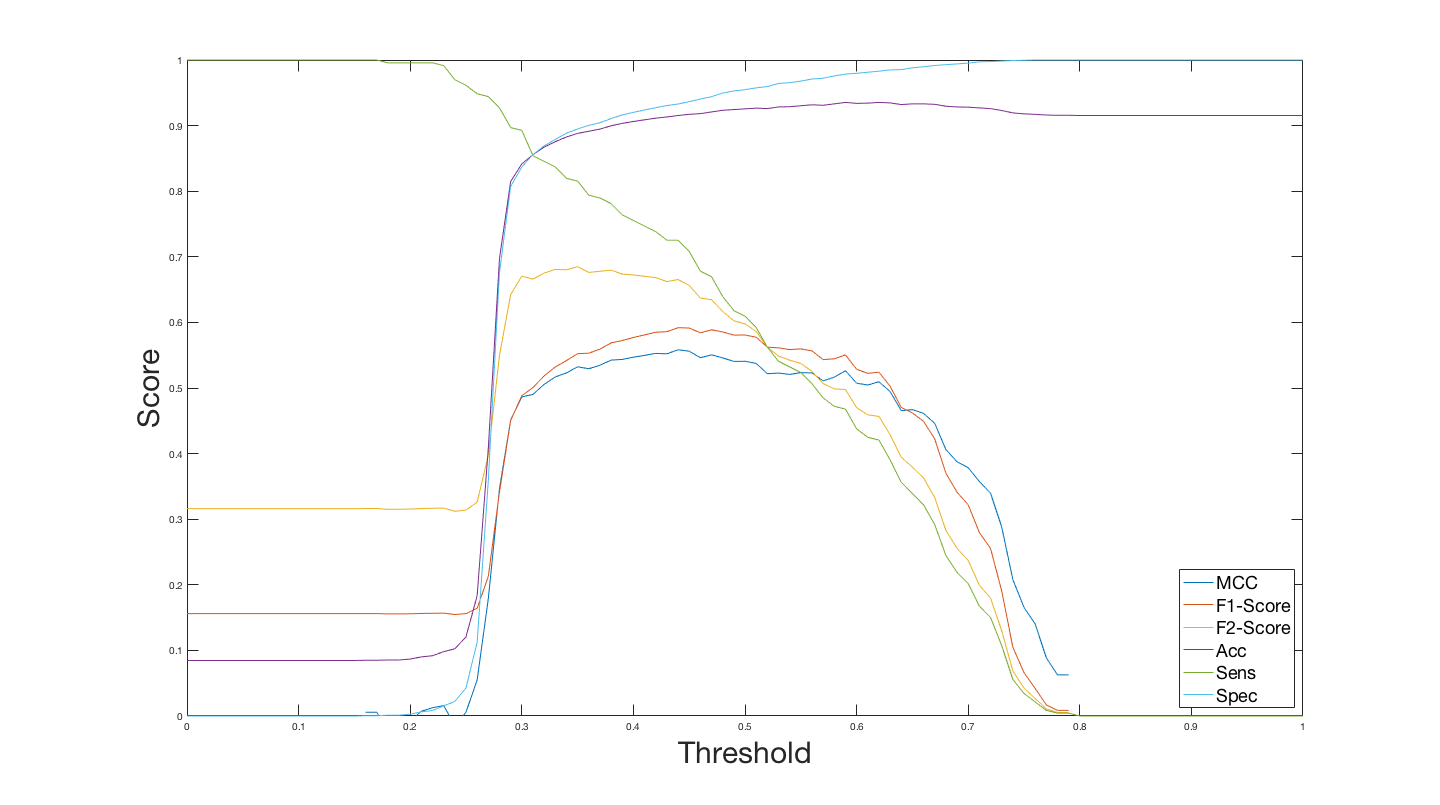
\includegraphics[width=\textwidth]{./pics/evaluation/treshold.png}
		\caption{Score-Threshold Abhängigkeit}
		\label{fig:threshold}
    \end{center}
\end{figure}

Wie man sehr gut erkennen kann gibt es einen Bereich zwischen $0.3$ und $0.6$ in der MCC und F2-Score gute Werte aufweisen. Da der F2-Score die falsch-negativen noch stärker bestraft konzentrierten wir uns hier noch einmal mehr auf diesen Qualitätsmaßstab. Auch eine hohe Sensitivität ist uns wichtig. Der F2-Score weist im Bereich $0.3$ und $0.45$ seine höchsten Werte auf, wobei der kleinste Threshold gleichzeitig die höchste Sensitivität ergibt. Es wäre also naheliegend einfach diesen Wert zu nehmen. Da die Spezifität zwischen dem Threshold $0.25$ und $0.3$ rapide ansteigt sollten ein gewisser Abstand zu diesem Bereich gewahrt werden. Somit entschieden wir uns den Threshold von den ursprünglichen $0.5$ auf $0.35$ herunterzusetzen. Damit halten wir genug Abstand von der extremen Änderung der Spezifität. Durch diese nun sensitivere Klassifizierung erhielten wir schließlich die Werte wie sie in Tabelle~\ref{final_scores} gelistet sind.

\begin{table}[htb!]
\begin{center}
\begin{tabular}{lllllllllll}
	\toprule
 	Threshold  & TP & FN & TN & FP & MCC & F2 & Acc & Sens & Spez\\
	\midrule
    $0.5$ & $142$&	$91$ &	$2406$ &	$114$ &	$0.54$ 	&$0.60$	&$0.93$	&$0.61$&	$0.95$ \\
	$0.35$ & $190$ &	$43$ &	$2255$ &	$265$ &	$0.55$ &	$0.68$&	$0.89$ &	$0.81$ & $0.89$\\
 \bottomrule
 \end{tabular}
 \end{center}
  \caption{Scores des Klassfizierers mit dem Threshold bei $0.35$}
 \label{tab:final_scores}
 \end{table}




\todo{Parameter für besten Trainingsdurchlauf}









